\documentclass[12pt]{article}
\usepackage[utf8]{inputenc} % Pacote para acentuação gráfica
%\usepackage[T1]{fontenc}
\usepackage[brazil]{babel} % nomes das estruturas em pt-br
%\usepackage{hyperref}
\usepackage{indentfirst} % indenta primeiro paragráfo após título
\usepackage{setspace} % pacote para alterar espaçamento entre linhas
%\setlength{\parindent}{1cm} % define o tamanho da indentação
%\setlength{\parskip}{0.3cm} % define o espaçamento vertical entre parágrafos
\usepackage[top = 2cm, left = 2cm, bottom = 2cm, right = 2cm]{geometry} % define as margens do documento
\usepackage{fancyhdr} % pacote para numeração de páginas
\usepackage{lipsum}  % Pacote para gerar texto de preenchimento
\usepackage{xcolor} % Definindo novas cores
\usepackage{graphicx} % para inserir figuras
\usepackage{float} % Força o posicionamento da figura
%\usepackage{amsmath} % Este pacote é necessário para usar símbolos matemáticos
\usepackage{gensymb} % símbolos trigonométricos
\usepackage{braket} % notações em álgebra "quântica"
\usepackage{amssymb} % Para acessar os símbolos do AMS


\definecolor{verde}{rgb}{0.25,0.5,0.35}
\definecolor{jpurple}{rgb}{0.5,0,0.35}
% Configurando layout para mostrar codigos Java
\usepackage{listings}
\lstset{
	language=Python,
	basicstyle=\ttfamily\small,
	keywordstyle=\color{jpurple}\bfseries,
	stringstyle=\color{red},
	commentstyle=\color{verde},
	morecomment=[s][\color{blue}]{/**}{*/},
	extendedchars=true,
	showspaces=false,
	showstringspaces=false,
	numbers=left,
	numberstyle=\tiny,
	breaklines=true,
	backgroundcolor=\color{cyan!10},
	breakautoindent=true,
	captionpos=b,
	xleftmargin=0pt,
	tabsize=4
}
\pagestyle{empty}

\begin{document}
	
\title{\textbf{{\Huge Notas em Computação Quântica}}} % Título
\author{\textbf{{\Large Ricardo Alvarenga}}} % Autor
\date{\textbf{{\Large 2024}}} % Data
\maketitle % Criar
\thispagestyle{empty} % oculta número da página

\begin{figure}[H]
	\centering
	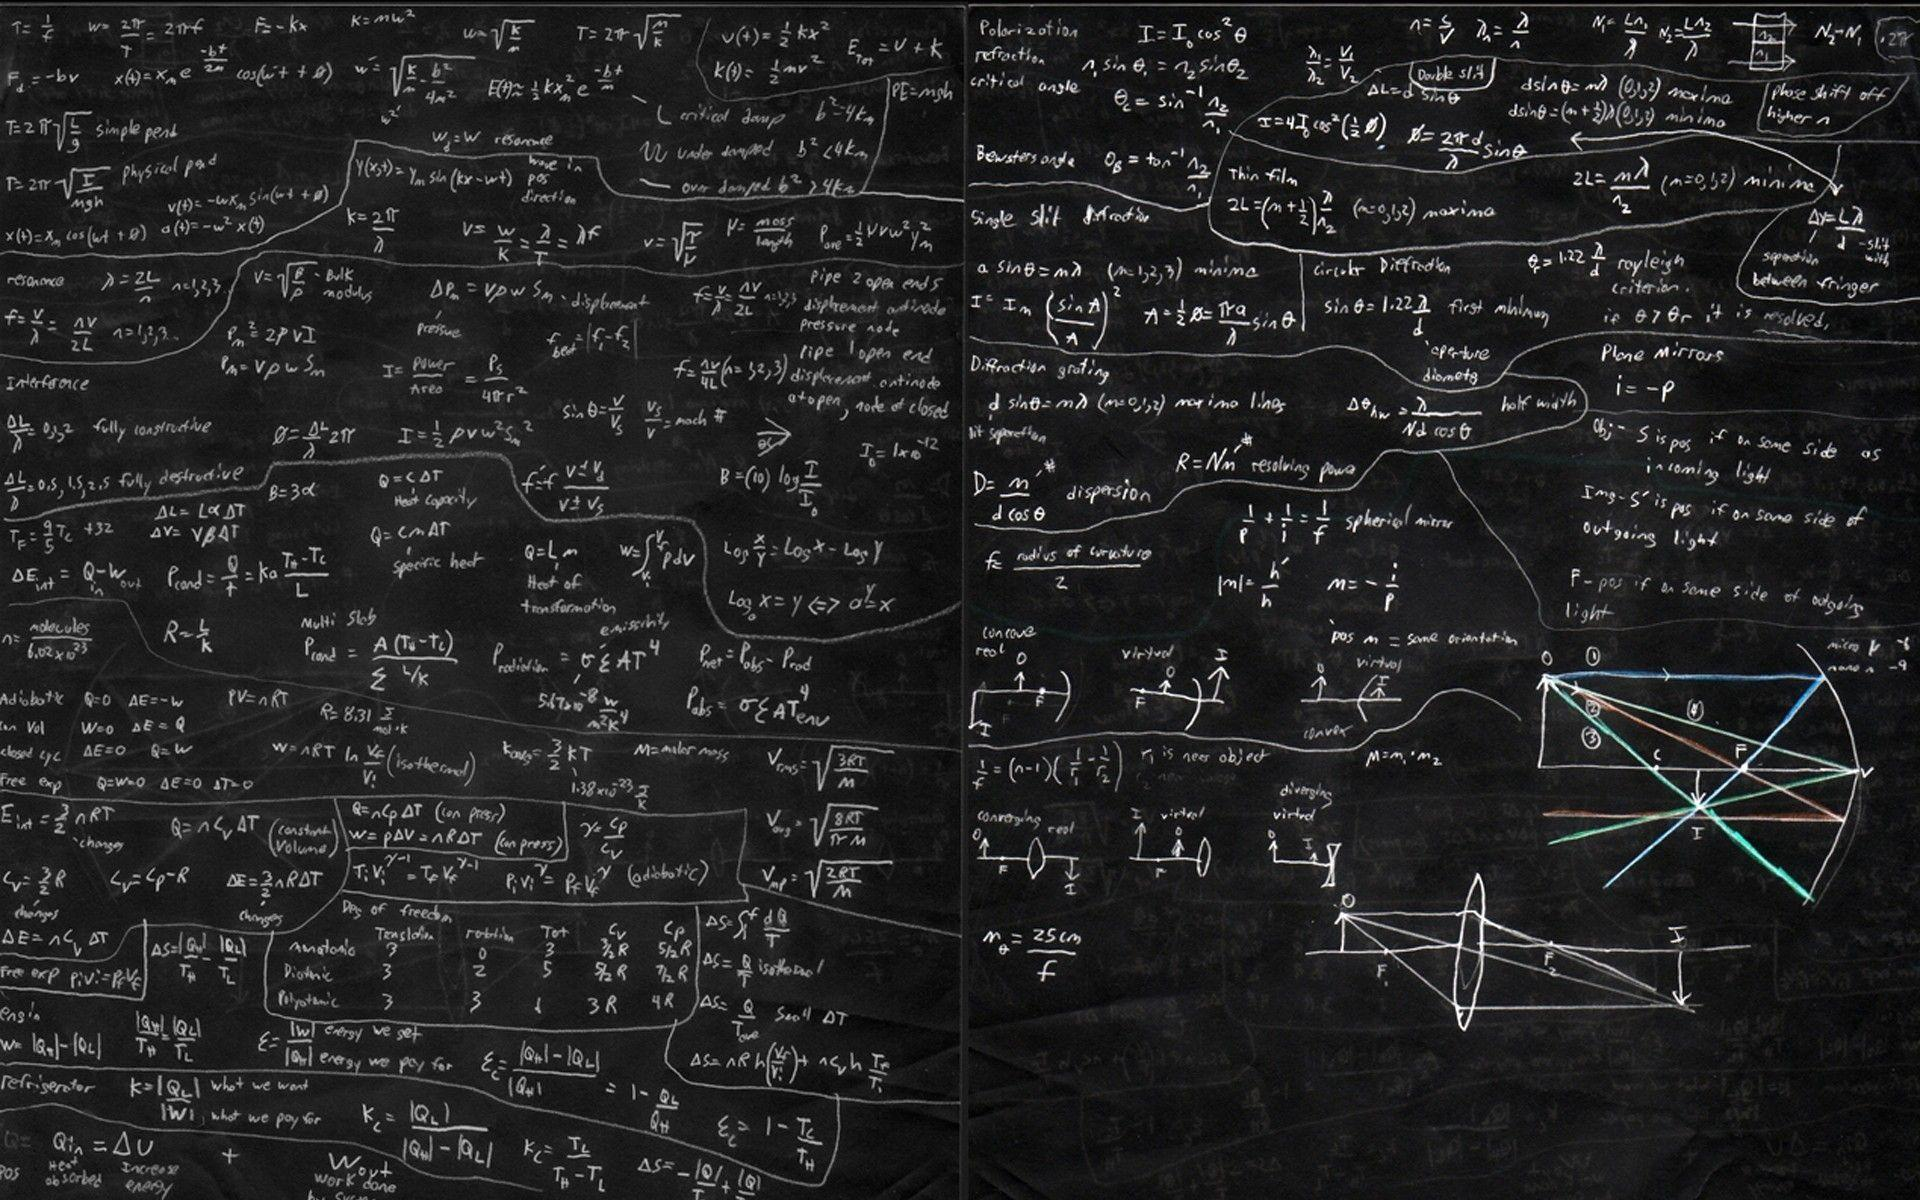
\includegraphics[width=1\linewidth]{figuras/wp5436123-quantum-physics-wallpapers}
\end{figure}


\newpage

\pagestyle{fancy}
\setcounter{page}{1} % reset contador de página
\pagenumbering{Roman}  % Altera número de página para números romanos
\tableofcontents % cria sumário
\newpage

\listoffigures % lista de figuras
\newpage


\pagestyle{fancy}
\fancyfoot[C]{\thepage} % Adiciona o número da página no centro do rodapé
\newpage

\setcounter{page}{1} % reset contador de página
\pagenumbering{arabic}
\pagestyle{fancy}
\fancyfoot[C]{\thepage}

% \twocolumn  % Inicia o ambiente de duas colunas

\onehalfspacing % espaçamento de 1,5 entre linhas

\section{Álgebra Linear}

\subsection{Vetores}

Vetores são seguimentos orientados (início em 0, 0) que estão sempre no plano cartesiano. Vetores são usados para representar grandezas escalares (massa, pressão, etc.) e grandezas físicas vetoriais (velocidade, força e deslocamento).

\begin{figure}[H]
	\centering
	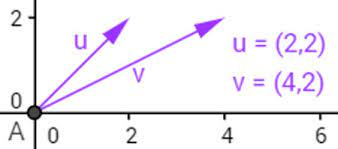
\includegraphics[width=.5\linewidth]{figuras/vetores_01}
	\caption[Vetores \textbf{u} e \textbf{v}]{Exemplos de Vetores, \textbf{u} e \textbf{v}}
	\label{fig:vetores01}
\end{figure}

\subsubsection{Vetores com duas dimensões - \( \mathbf{R}^{2} \)}

\(x, y\) podem assumir qualquer valor \textit{Real}.

\begin{figure}[H]
	\centering
	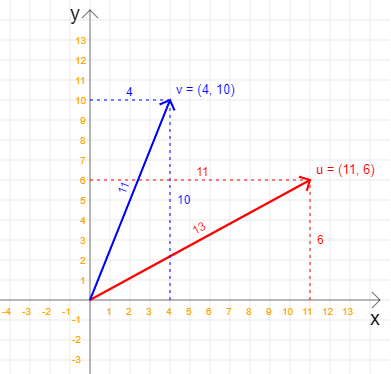
\includegraphics[height=.45\textheight]{figuras/vetores_02}
	\caption[Vetores em \( \mathbf{R}^{2} \)]{Vetores em \( \mathbf{R}^{2} (x, y)\)}
	\label{fig:vetores02}
\end{figure}

\newpage

\subsubsection{Vetores com três dimensões - \( \mathbf{R}^{3} \)}

\(x, y, z\) podem assumir qualquer valor \textit{Real}.

\begin{figure}[H]
	\centering
	\includegraphics[width=0.5\linewidth]{"figuras/vetores R3"}
	\caption[Vetores em \( \mathbf{R}^{3} \)]{Vetores em \( \mathbf{R}^{3} (x, y, z)\)}
	\label{fig:vetores-r3}
\end{figure}

\subsubsection{Vetores com \textit{n} dimensões - \( \mathbf{R}^{n} \)}

Os vetores com \textit{n} dimensões são de difícil (ou impossível) representação gráfica.

Um vetor \( \mathbf{R}^{4} \) é indicado da seguinte forma: \( \mathbf{R}^{4} (x, y, z, w)\)

\subsubsection{Como colocar um vetor no plano \( \mathbf{R}^{3} \)(x, y, z)}

Veja na figura \ref{fig:vetor r3} o vetor \(u = (2,4,3)\).

\begin{figure}
	\centering
	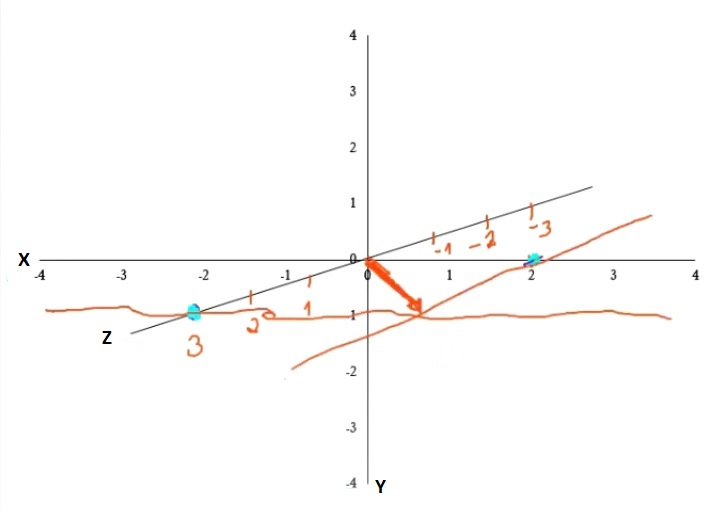
\includegraphics[width=0.7\linewidth]{figuras/R3}
	\caption[Vetor em \( \mathbf{R}^{3} \)]{Vetor em \( \mathbf{R}^{3} \)}
	\label{fig:vetor r3}
\end{figure}

\subsubsection{Tipos de vetores}

\singlespacing
\begin{itemize}
	\item Vetor Nulo: Todos valores iguais a zero. Ex: \(v = (0,0,0)\)
	\item Vetor simétrico ou oposto: Ocorre quando dois vetores são opostos e contêm o mesmo módulo e mesma direção. Ex: \(v = (x,y), -v = (-x,-y)\)
	\item Vetor unitário: Possui módulo (tamanho) igual a 1. \(|v| = 1\)
	\item Vetores colineares ou paralelos: Ocorrem quando dois vetores tiverem a mesma direção, na mesma reta ou retas paralelas.
	\item Vetores coplanares: Quando dois vetores fazem parte de um mesmo plano.
\end{itemize}
\onehalfspacing
\pagebreak

\subsubsection{Igualdade de vetores}

Dois vetores serão iguais se: 

\singlespacing
\begin{itemize}
	\item \(x_{1} = x_{2}\)
	\item \(y_{1} = y_{2}\)
	\item \(z_{1} = z_{2}\) vetores em \(R^{3}\)
	\item \(w_{1} = w_{2}\) vetores em \(R^{4}\)
\end{itemize}
\onehalfspacing

\(u = (3, x + 4)\) \(v = (3, 8)\) se \(x = 4\) os vetores serão iguais.

Sejam: \(u = (x-1, 3)\), \(v = (3, 2y-1)\). Determine o valor de \(x\) e \(y\) para que \(u = v\).

\(x = 4\), \(y = 2\)

\subsubsection{Soma de vetores}

Para realizar a soma de dois vetores temos que efetuar a soma de cada elemento com seu correspondente.

Exemplo:

\(u = (2, 3)\), \(v = (5, 6)\)

\(u + v = (7, 9)\)

\subsubsection{Subtração de vetores}

\(A = (-1, 2)\)   \(B = (2,1)\). \(v = $\overrightarrow{AB}$\) o vetor está "perdido" no plano cartesiano. Para corrigir isso, realizamos a subtração:

\(B - A = (2, 1) - ( -1, 2) = (3, -1)\). Que resulta no vetor \(t = (3, -1)\), conforme figura \ref{fig:subtracaovetores01}.

Outro exemplo: Dois vetores \(u = (-1, 3)\) e \(v = (10, 20)\), a subtração \(u - v\) resulta em \((-11, -17)\).

Sejam \(u\) e \(v\) vetores no \( \mathbf{R}^{n}\)\cite{lipschutz-algebra}: \(u=(a_{1}, a_{2},...,a_{n})\) e \(v=(b_{1}, b_{2},...,b_{n})\)

\(u-v = (a_{1} - b_{1}, a_{2}-b_{2},...,a_{n}-b_{n})\).

\begin{figure}
	\centering
	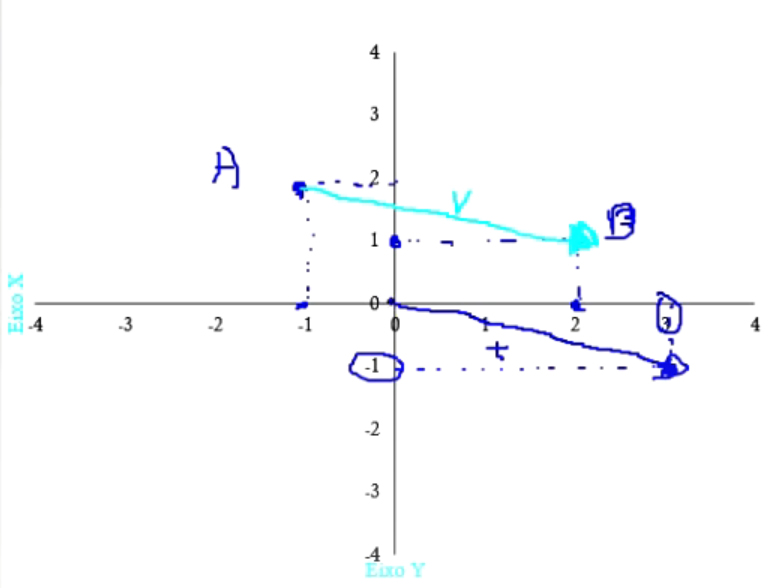
\includegraphics[width=0.7\linewidth]{figuras/subtracao_vetores_01}
	\caption[Subtração de Vetores]{Subtração de Vetores}
	\label{fig:subtracaovetores01}
\end{figure}

\subsubsection{Multiplicação de dois vetores (Produto Escalar)}

Assim como na soma e subtração de vetores, podemos multiplicar vetores. O nome correto deste tipo de operação é \textit{Produto Escalar}.

Sejam \(u\) e \(v\) vetores no \( \mathbf{R}^{n}\): \(u=(a_{1}, a_{2},...,a_{n})\) e \(v=(b_{1}, b_{2},...,b_{n})\)

\(u*v = (a_{1} * a_{2} + b_{1} * b_{2} ,..., + a_{n} * b_{n})\).

Exemplo: \(u = (1,2)\), \(v = (5, 3)\)
Então: \(u*v = (1, 2, 3, 4) * (5, 3, 1, 4) = (5 + 6 + 3 + 16) = 30\)

\subsubsection{Multiplicação por um escalar}

Multipliacação por um escalar é multiplicar um número por um vetor.

Sejam: \(t = (x_{1}, x_{2}, ..., x_{n})\) e um número \(a\)

Temos: \(at = a(x_{1}, x_{2}, ..., x_{n}) = (a*x_{1}, a*x_{2}, ..., a*x_{n})\)

Exemplo:

\(u = (4, 5)\) e \(a = 2\), \(au = 2(4, 5) = (8, 10)\)

\subsubsection{Módulo/Norma (Norm) de um vetor}

A norma ou módulo de um vetor é o comprimento desse vetor, que pode ser calculado por meio da distância de seu ponto final até a origem.

A norma de \( u \) é denotada por \( \| u \| \).

Considerando o vetor \(u = (a_{1}, a_{2}, ..., a_{n})\), calculamos sua norma, ou módulo, da seguinte forma\cite{lipschutz-algebra, anton2012algebra}: \( \|u\| = \sqrt{u*u} = \sqrt{a_{1}^2 + a_{2}^2 + ... + a_{n}^2} \) 

Exemplo: \(v = (5, 6)\), \(\|v\| = \sqrt(v*v) = \sqrt(5,6)*(5,6) = \sqrt{61}\)

ou de forma direta:

\(\|v\| = \sqrt{(5^2+6^2)} = \sqrt{61}\)


Se \(\|u\| = 1\), temos um vetor unitário.

\subsubsection{Ângulo entre dois vetores (Ângulo $\Theta$ de dois vetores)}

Considerando dois vetores que partem do mesmo ponto, o ângulo entre eles é representado por $\Theta$. O ângulo $\Theta$ é dado por:

\(cos \Theta\ = \frac{u * v}{\|u\|*\|v\|}\)

Exemplo:

Sendo os vetores \(u = (2,2)\) e \(v=(0, -2)\), encontre o ângulo $\Theta$:

\(cos \Theta\ = \frac{u * v}{\|u\|*\|v\|} = \frac{-4}{\sqrt(8)*2} = \frac{-2}{\sqrt{8}}=\frac{-2}{\sqrt{2}*\sqrt{4}}=\frac{\frac{-2}{2}}{\sqrt{2}} = \frac{-1}{\sqrt{2}} = \frac{-1}{\sqrt{2}} * \frac{\sqrt{2}}{\sqrt{2}} = \frac{-\sqrt{2}}{2} = 135\degree\)

\subsubsection{Vetores colineares}

Dois vetores são colineares (paralelos), quando:

\(v = (x_{1}, y_{1})\) e \(t = (x_{2}, y_{2})\)

\(\frac{x_{1}}{x_{2}} = \frac{y_{1}}{y_{2}} = a\)
\\

Exemplo: Verifique se \(u\) e \(v\) são colineares, sendo \(u = (-3, 2)\) e \(v=(6,-4)\)

\(\frac{-3}{6} = -\frac{1}{2}\) e \(\frac{2}{-4} = -\frac{1}{2}\) então: \(a = -\frac{1}{2}\)

\subsubsection{Ortogonalidade de dois vetores}

Considerando dois vetores coplanares (em \(R^{2}\)), eles serão ortogonais se o $\Theta$, entre eles, for 90\degree.

Matematicamente: \(u * v = 0\)

Exemplo: Verifique se os vetores \(u = (1, 2)\) e \(v = (-2, 1)\), são ortogonais:

\(u * v = (1 * -2 + 2 * 1) = (-2 + 2) = 0\)


\subsubsection{Vetores perpendiculares}

Dois vetores, em \(R^{n}\) com \(n \geq 3\), são perpendiculares entre si, se o seu produto escalar for igual a zero.

\subsubsection{Projeção ortogonal entre dois vetores}

A projeção ortogonal de um vetor \(v\) sobre outro vetor \(u\) é a componente de \(v\) na direção de \(u\). Essa projeção é chamada de "ortogonal" porque é perpendicular ao vetor de referência \(u\).

A projeção ortogonal de \(v\) sobre \(u\), denotada por \(proj_{u}(v)\), é calculada usando a seguinte fórmula: \(proj_{u}(v) = \left( \frac{u \cdot v}{\|u\|^2} \right) u\)


Onde:\(u * v \) é o produto escalar entre os vetores \( u \) e \( v \).
- \( \| u \| \) é a norma (ou magnitude) do vetor \( u \).

Essa fórmula nos diz que a projeção ortogonal de \( v \) sobre \( u \) é obtida multiplicando o vetor \( u \) pela fração \(\frac{u*v}{\|u\|^2}\), que é a magnitude da projeção de \(v \) na direção de \(u\).




\section{Teste}

O estado quântico $\ket{\psi}$ é representado como um ket vector.

$\ket{0}$, $\ket{1}$

$\alpha_{1}, \alpha_{2}, \alpha_{3}$

\(\alpha_{4}, \alpha_{5}, \alpha_{6} \)

O conjunto dos números reais é denotado por $\mathbb{R}$.


% \lipsum[1-10]  % Exemplo de texto de preenchimento

\newpage
%Biblioteca
\bibliographystyle{unsrt} %estilo
\bibliography{./referencias/referencias}
	
\end{document}